\chapter{Evaluation}
\label{sec:evaluation}

Chapters~\ref{sec:derivative-parser} and~\ref{sec:partial-derivative-parser}
developed four parser combinations -- \texttt{deriv\_std},
\texttt{deriv\_bc}, \texttt{pderiv\_std}, \texttt{pderiv\_bc} -- each
claimed to compute either the POSIX or the Greedy $\geq_r$-ordered parse
tree, by four structurally different constructions. This chapter
verifies those claims empirically: Section~\ref{sec:testing-strategy}
describes how the test suite checks the four parsers, and the three
Boolean matchers of Chapter~\ref{sec:derivatives}, against each other
and against the paper's own worked examples;
Section~\ref{sec:dataset-preparation} describes how a corpus of
real-world regular expressions was assembled to test and benchmark
against, alongside the synthetic patterns used elsewhere in this
thesis; Section~\ref{sec:correctness-verification} reports the results
of that testing; and Section~\ref{sec:performance-analysis} measures
where the four parsers' costs actually diverge from each other, on both
the synthetic and real-world workloads.



\section{Compared Engines}
\label{sec:compared-engines}

The primary object of comparison in this chapter is the four parser
combinations against \emph{each other} -- two POSIX, two Greedy, one
tree-building and one bit-coded within each pair
(Chapters~\ref{sec:derivative-parser}-\ref{sec:partial-derivative-parser})
-- since that internal comparison is what this thesis's own theoretical
claims (POSIX-correctness, Greedy/POSIX agreement on membership, the
tree-vs-bit-coded performance trade-off) are actually about. A second,
external comparison against established regular expression engines is
motivated in Chapter~\ref{sec:motivation} and positions these results
relative to the wider field. It is implemented as an optional,
feature-gated addition to this codebase (Rust's \texttt{regex} crate as
an ordinary optional dependency; Google's RE2 via a small C++ shim over
its own API, since RE2 offers no C API of its own) rather than a default
one, specifically so that the default build stays free of any external
regular-expression engine dependency -- \texttt{cargo build}/\texttt{cargo
test}/\texttt{cargo bench} never touch either engine unless the
\texttt{external-engines} feature is explicitly enabled.
Section~\ref{sec:comparison-existing-engines} reports and discusses the
resulting numbers; what follows briefly positions both engines
conceptually, since that section refers back to this framing.

\subsection{Rust's \texttt{regex} Crate}
\label{sec:rust-regex-crate-eval}

Rust's \texttt{regex} crate compiles a pattern to a Thompson-construction
NFA and simulates it without backtracking, guaranteeing linear-time
matching in the input length independent of the pattern -- the same
automaton-based guarantee Chapter~\ref{sec:motivation} attributes to
finite-automata approaches generally. Its disambiguation policy is
leftmost-first, matching Section~\ref{sec:greedy-leftmost}'s Greedy
order rather than POSIX leftmost-longest; it offers no POSIX mode. This
makes it a natural comparison point for this thesis's Greedy parsers
(\texttt{pderiv\_std}/\texttt{pderiv\_bc}) specifically, on both
performance and, since both claim the same disambiguation policy,
parse-tree agreement -- an even more direct check than the
membership-only agreement this thesis's own Greedy/POSIX comparison
already establishes (Section~\ref{sec:correctness-verification}).

\subsection{RE2}
\label{sec:re2-eval}

Google's RE2 is likewise automaton-based (Thompson NFA compiled lazily
to a DFA on demand), explicitly designed to avoid the exponential
backtracking blowup of backreference-supporting engines
\citep{re2,cox2007}. Unlike Rust's \texttt{regex} crate, RE2 supports an
explicit POSIX leftmost-longest mode alongside its default Perl-style
leftmost-first mode, making it a comparison point for \emph{both}
disambiguation policies studied in this thesis, in one engine, depending
on which mode is selected.



\section{Testing Strategy}
\label{sec:testing-strategy}

The test suite is split, following ordinary Rust convention, into unit
tests (\texttt{\#[cfg(test)] mod tests} blocks inside the \texttt{src/}
files they exercise, testing private helper functions alongside public
ones) and integration tests (\texttt{tests/}, exercising only the public
API each parser or matcher module exposes). \texttt{tests/common/mod.rs}
factors out what is shared across the integration suites: the two
worked examples from the paper, \texttt{paper\_r1} and \texttt{paper\_r2}
(Section~\ref{sec:parse-trees-as-evidence}), and two assertion helpers,
\texttt{assert\_round\_trip} (checking \texttt{flatten(parse(r,w)) == w},
i.e.\ that a produced parse tree is actually evidence for the word it
was built from) and \texttt{assert\_parsers\_agree} (comparing two
\texttt{Option<ParseTree>} results with a labeled failure message
identifying which two implementations disagreed).

\paragraph{The agreement-testing pattern.} Section~\ref{sec:matcher-selection}
already introduced the underlying idea for the three Boolean matchers:
give independently-written implementations a common interface, run them
on the same input, and treat disagreement as a bug in one of the
implementations rather than an ambiguity in what the answer should be.
This thesis's test suite applies the identical pattern one level up, at
every layer that has more than one implementation of the same
specification -- \texttt{match\_naive}/\texttt{match\_deriv}/\texttt{match\_pderiv}
against each other; \texttt{parse\_recursive} against \texttt{parse\_loop}
(same construction, same algorithm, different recursion strategy,
Section~\ref{sec:recursive-vs-loop}); all four parser combinations
against each other, restricted to membership (\texttt{Option::is\_some})
where POSIX and Greedy are known to disagree on tree shape, and to exact
tree equality where they are not; and, within the two Greedy parsers
specifically, \texttt{pderiv\_std} against \texttt{pderiv\_bc} for exact
tree equality unconditionally, since both claim to compute the
identical policy with no legitimate source of disagreement between them
(Section~\ref{sec:pderiv-std-theory-rust}).

\paragraph{Differential fuzzing.} Where the input space is too large to
enumerate by hand, agreement is checked instead over many
pseudo-randomly generated regular expressions and inputs, using a small
self-contained xorshift generator (avoiding an external
dependency purely for reproducible test-time randomness) to build
\texttt{Regex} trees of bounded depth and words of bounded length over a
small alphabet, then asserting agreement -- exactly the same pattern as
the hand-picked test cases above, just applied at volume rather than to
individually chosen examples. \texttt{tests/test\_pderiv\_std.rs}'s
\texttt{fuzz\_std\_matches\_bitcoded\_exactly}, checking
\texttt{pderiv\_std} against \texttt{pderiv\_bc} over 20{,}000 generated
cases, and \texttt{fuzz\_membership\_agrees\_with\_posix}, checking
membership agreement with \texttt{parse\_recursive} over a further
10{,}000, are the two most significant instances -- as
Section~\ref{sec:pderiv-std-theory-rust} already noted, in the absence
of a reference construction for either Greedy partial-derivative parser,
this volume of agreement between two independently-shaped
implementations is the strongest correctness evidence available for
either of them.



\section{Dataset Preparation}
\label{sec:dataset-preparation}

The synthetic patterns used throughout this thesis -- \texttt{paper\_r1},
\texttt{paper\_r2}, the pathological $(a^{*})^{*}$-style expressions of
Section~\ref{sec:membership-overview} -- are deliberately small and
hand-constructed, chosen to isolate one specific algorithmic property at
a time. They say little about how any of the four parsers behaves on the
regular expressions people actually write. Mamouras et al.'s
disambiguation-robustness study \citep{mamouras2024} motivates closing
that gap: it studies exactly the POSIX-versus-Greedy question this
thesis studies, via real Snort/Suricata intrusion-detection signatures,
and finds concrete real-world patterns where the two policies visibly
diverge. That paper provides no public dataset artifact of its own, so
this thesis's corpus was independently assembled from three families of
real-world regular expression sources chosen to cover different
"shapes" of real regex use, not three samples of the same thing:

\begin{itemize}
  \item \textbf{Snort/Suricata} network intrusion-detection signatures
  (\texttt{pcre:"..."} rule options, sourced from the Emerging Threats
  Open ruleset) -- literal-heavy, moderate complexity, the closest of
  the three to "everyday" regex use.
  \item \textbf{SpamAssassin} email spam-filtering rules
  (\texttt{body}/\texttt{header} Perl-regex rules) -- content matching
  over unstructured text, a different shape than network signatures.
  \item \textbf{RegexLib} crowd-sourced general-purpose patterns
  (validators, extractors) -- the opposite end, where chained lookahead
  assertions are idiomatic, stress-testing the frontend's rejection path
  hardest of the three.
\end{itemize}

\paragraph{Extraction.} Each source embeds its patterns in a different
surrounding syntax, so each needs its own extractor
(\texttt{examples/extract\_dataset.rs}): Suricata's rule lines carry a
\texttt{pcre:"/PATTERN/FLAGS";} option; SpamAssassin's carry a bare
\texttt{body}/\texttt{header NAME =~ /PATTERN/FLAGS} without the
Suricata's trailing-quote convention; RegexLib's sample file lists plain
patterns directly, one (possibly multi-line) entry per blank-line-delimited
block. All three converge on the same \texttt{/PATTERN/FLAGS} PCRE
delimiter convention once extracted, parsed by
\texttt{frontend::parse\_pcre\_rule} -- including the case-insensitive
\texttt{i} flag, applied by case-folding every literal character in the
translated \texttt{ExtPat} to an \texttt{Any} of both cases
(Section~\ref{sec:regex-rust-implementation}'s frontend, not covered
further in this thesis, since it concerns surface syntax rather than
the derivative-based algorithms this thesis is about) rather than as a
runtime matching option, since \texttt{Regex} itself has no
case-insensitivity concept.

\paragraph{Filtering.} Real rules routinely use constructs no
derivative-based engine over the six-constructor \texttt{Regex} of
Section~\ref{sec:regex-rust-implementation} can express at all --
backreferences and lookaround assertions describe languages that are
not regular in the formal sense this thesis's entire construction
depends on. \texttt{parse\_pcre\_rule} rejects both outright with a
descriptive error rather than silently mis-parsing them, and
\texttt{extract\_dataset} tallies every rejection by cause
(\texttt{backreference}, \texttt{lookaround}, or \texttt{other} --
chiefly bound expressions such as \texttt{\{1586,\}} that would unroll
past this frontend's repetition cap, and a handful of unsupported
\texttt{(?...)}~group syntaxes). Re-running this pipeline against the
tracked raw sources gives the current triage:

\begin{center}
\begin{tabular}{lrrrrr}
\hline
Format & Extracted & Accepted & Backreference & Lookaround & Other \\
\hline
Suricata & 231 & 209 (90.5\%) & 5 & 11 & 6 \\
SpamAssassin & 82 & 69 (84.1\%) & 1 & 11 & 1 \\
RegexLib & 499 & 407 (81.6\%) & 8 & 55 & 29 \\
\hline
\textbf{Total} & \textbf{812} & \textbf{685 (84.4\%)} & \textbf{14} & \textbf{77} & \textbf{36} \\
\hline
\end{tabular}
\end{center}

Lookaround dominates the rejections and is concentrated almost entirely
in RegexLib, matching that family's idiomatic use of chained
assertions; Suricata and SpamAssassin reject mostly on the same handful
of negative-lookahead idioms (guarding against one specific following
word). The accepted 685 patterns, deduplicated across all three formats
into \texttt{data/corpus\_patterns.txt} (665 lines after deduplication),
are what Section~\ref{sec:benchmark-results}'s dataset benchmark
actually runs against.

\paragraph{Unanchored matching.} Real rules are \emph{written} as
search patterns -- a Suricata rule fires on seeing a match anywhere in a
packet payload, not on the payload being exactly that pattern -- so they
are parsed for substring search via
\texttt{frontend::parse\_dataset\_pattern}/\texttt{parse\_pcre\_rule}
rather than the full-string-equality \texttt{parse\_pattern} used
elsewhere in this thesis's own examples: an unanchored core pattern is
padded with \texttt{(alphabet)*} on whichever side lacks an explicit
\texttt{\^{}}/\texttt{\$} anchor, itself an ordinary \texttt{Star} over
a 98-way alternation with no special status in the parser layer, and
therefore a real subexpression contributing to whatever cost that
padding adds -- part of why real dataset patterns, run unanchored the
way they have to be, are measurably bigger and expose scaling behavior
the small synthetic patterns of Section~\ref{sec:pathological-inputs}
do not by themselves.

\paragraph{What this dataset does not (yet) give.} The corpus was
triaged for "does it parse at all," not for "does POSIX visibly diverge
from Greedy on this pattern the way \texttt{paper\_r1}/\texttt{paper\_r2}
do" -- unlike Mamouras et al.'s own disambiguation-robustness analysis
\citep{mamouras2024}, this thesis does not (yet) identify which, if any,
of the 685 accepted real-world patterns are themselves
disambiguation-non-robust in their sense. Combining this dataset with
their static-analysis technique to find such patterns automatically, or
constructing inputs that provoke visible POSIX/Greedy divergence on the
existing corpus directly, is a natural extension of this evaluation left
to future work (Section~\ref{sec:further-performance-optimizations}).



\section{Correctness Verification}
\label{sec:correctness-verification}

\subsection{Paper Examples Reproduced}
\label{sec:paper-examples-reproduced}

Both worked examples from Sulzmann and Lu's paper are reproduced as
executable tests rather than only as the manual derivations of
Sections~\ref{sec:disambiguation-problem} and~\ref{sec:posix-longest-leftmost}:
\texttt{parse\_recursive\_paper\_r1\_on\_ab} and
\texttt{parse\_recursive\_paper\_r2\_on\_ab}
(\texttt{tests/test\_deriv\_std.rs}) assert the exact POSIX tree shape
derived by hand in Section~\ref{sec:posix-longest-leftmost};
\texttt{paper\_r1\_computes\_greedy\_not\_posix} and
\texttt{paper\_r2\_computes\_greedy\_not\_posix}
(\texttt{src/parsers/pderiv\_bc/parse.rs}) assert both the Greedy tree
shape of Section~\ref{sec:greedy-leftmost} \emph{and} that it disagrees
with the POSIX answer on the identical input -- encoding the divergence
itself, not merely each answer separately, as the property under test.
Every one of these four assertions currently passes, confirming this
implementation reproduces both documented policies exactly on the
paper's own examples.

\subsection{Cross-Implementation Equivalence}
\label{sec:cross-implementation-equivalence}

Following the agreement-testing strategy of
Section~\ref{sec:testing-strategy}, the full test suite checks, and at
the time of writing passes, agreement at every layer this thesis
introduces more than one implementation of the same specification:

\begin{itemize}
  \item \texttt{match\_naive} = \texttt{match\_deriv} = \texttt{match\_pderiv}
  on membership, across the hand-picked cases of
  \texttt{tests/test\_matchers.rs}.
  \item \texttt{parse\_recursive} and \texttt{parse\_loop} produce
  identical parse trees on every shared test case
  (Section~\ref{sec:recursive-vs-loop}), including
  \texttt{recursive\_traced\_and\_loop\_traced\_agree\_on\_all\_paper\_examples}
  comparing full derivation traces, not just final answers.
  \item \texttt{deriv\_bc} agrees with \texttt{deriv\_std} (via
  \texttt{parse\_recursive}) on every shared test case
  (\texttt{bitcoded\_agrees\_with\_recursive}, \texttt{tests/test\_deriv\_bc.rs}),
  the empirical counterpart of Section~\ref{sec:derivative-parser}'s
  claim that both compute the identical POSIX tree by different means.
  \item \texttt{pderiv\_std} and \texttt{pderiv\_bc} agree exactly, not
  just on membership, on every hand-picked and fuzzed case
  (Section~\ref{sec:testing-strategy}).
  \item All four parser combinations agree on membership wherever POSIX
  and Greedy are not known to diverge, and the two POSIX parsers
  (\texttt{deriv\_std}, \texttt{deriv\_bc}) and two Greedy parsers
  (\texttt{pderiv\_std}, \texttt{pderiv\_bc}) each agree exactly with
  their own policy-mate on tree shape -- exercised directly by the CLI's
  \texttt{-{}-parser all} comparison mode
  (\texttt{src/cli/parser.rs}), which reports all three checks
  side by side for a given regex/input pair on demand.
\end{itemize}

No disagreement has been observed in any of these checks against the
current implementation; a regression in any one parser would show up
first as a failure here, in the specific pairing that parser
participates in, before it could show up as an incorrect answer with no
diagnosis of which implementation is at fault.



\section{Performance Analysis}
\label{sec:performance-analysis}

\subsection{Stack Depth: Recursive vs.\ Iterative Construction}
\label{sec:stack-depth}

\texttt{parse\_recursive}'s native recursion
(Section~\ref{sec:recursive-vs-loop}) ties its stack usage directly to
input length, with no guaranteed tail-call optimization in Rust to
eliminate it -- unlike \texttt{parse\_loop}, which keeps the derivative
sequence on the heap as an explicit \texttt{Vec<Regex>} instead.
\texttt{examples/demo\_crash.rs} measures this difference directly:
paired with a minimal subprocess worker (\texttt{demo\_crash\_worker.rs},
isolating each trial so a stack overflow terminates only the worker, not
the measurement harness itself), it binary-searches for the longest
\texttt{"a"}-repeated input each construction survives against
$a^{*}$, in both debug and release builds -- release binaries typically
surviving considerably longer inputs than debug builds of the identical
code, since debug builds carry heavier per-frame bookkeeping (overflow
checks, unoptimized stack frame layout) that consumes stack budget
\texttt{parse\_recursive}'s recursion is otherwise unaware of. The exact
crash threshold is a property of the platform's configured stack size
and the build profile, not of the algorithm, and is reproduced directly
via \texttt{cargo run --example demo\_crash} (and, in release mode,
\texttt{-{}-release}) rather than hard-coded here as a fixed number this
thesis cannot guarantee holds on a reader's own machine; what the two
constructions guarantee \emph{qualitatively} does not depend on the
platform: \texttt{parse\_loop} survives strictly longer inputs than
\texttt{parse\_recursive} on identical hardware and build configuration,
in exchange for the heap allocation Section~\ref{sec:heap-allocation}
discusses next.

\subsection{Heap Allocation: \texttt{deriv\_std} vs.\ \texttt{deriv\_bc}}
\label{sec:heap-allocation}

\texttt{deriv\_std}'s two-pass construction
(Section~\ref{sec:core-algorithm}) necessarily retains its entire
forward-pass sequence -- explicitly as a \texttt{Vec<Regex>} in
\texttt{parse\_loop}, implicitly as call-stack frames in
\texttt{parse\_recursive} -- until the backward pass consumes it,
alongside the \texttt{Box}-indirected recursive \texttt{Regex} nodes
(Section~\ref{sec:regex-rust-implementation}) each intermediate
expression itself allocates. \texttt{deriv\_bc}
(Section~\ref{sec:bitcoded-optimization-theory}) allocates no such
sequence: each step's \texttt{ARegex} (itself no more heap-indirected
than a \texttt{Regex} of the same shape, since it mirrors
\texttt{Regex}'s own \texttt{Box} usage one to one) replaces the
previous one in place, and the accumulated per-node
\texttt{Vec<bool>}s that carry parse-tree information are typically
short relative to a fully-materialized \texttt{ParseTree}. This is the
"incremental" single-pass promise of
Section~\ref{sec:bitcoded-optimization-theory} realized concretely:
fewer live allocations at any one point during parsing, at the cost of
the \texttt{decode} step (Section~\ref{sec:decode}) needed once, at the
very end, to turn accumulated bits back into an ordinary
\texttt{ParseTree} -- work \texttt{deriv\_std} instead spreads across its
explicit backward pass.

\subsection{Derivative-Based vs.\ Partial-Derivative-Based}
\label{sec:deriv-vs-pderiv-performance}

The comparison's other axis, orthogonal to
Section~\ref{sec:heap-allocation}'s tree-vs-bit-coded question, is
Brzozowski's single evolving expression (Section~\ref{sec:brzozowski-derivatives})
against Antimirov's evolving \emph{set} of residuals
(Section~\ref{sec:antimirov-partial-derivatives}): \texttt{deriv\_std}/
\texttt{deriv\_bc} maintain exactly one expression at every step,
however large its internal syntax tree, where \texttt{pderiv\_std}/
\texttt{pderiv\_bc} maintain a frontier whose size varies with how
ambiguous the pattern is against the input consumed so far, bounded by
Antimirov's finiteness result (Section~\ref{sec:antimirov-partial-derivatives})
but not by a constant independent of the pattern. \texttt{benches/bench\_posix.rs}
measures both axes together across the same small pattern/input pairs,
comparing all five internal constructions (\texttt{parse\_recursive},
\texttt{parse\_loop}, \texttt{parse\_bitcoded}, \texttt{parse\_pderiv\_std},
\texttt{parse\_pderiv\_bc}) side by side via Criterion benchmark groups
named for the property under test (\texttt{small\_patterns},
\texttt{scaling\_a\_star}, \texttt{deep\_expression},
\texttt{ambiguous\_star\_a\_or\_aa}). Exact numbers are a property of the
benchmarking machine and drift over a fixed document cannot track --
\texttt{docs/testing/BENCHMARKS.md} documents how to reproduce a current
run -- but one representative run's shape, from \texttt{deep\_expression}
(nested concatenation, depth $50$ to $1000$), is worth showing directly,
since it makes both axes above visible in one plot:

\begin{center}
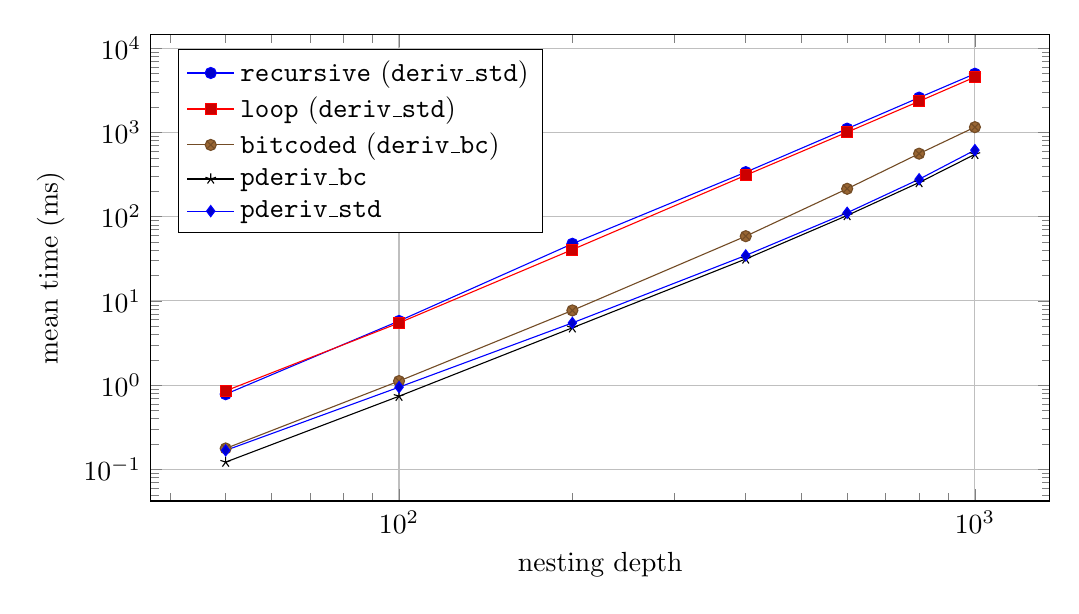
\begin{tikzpicture}
\begin{axis}[
  width=13cm, height=7.5cm,
  xlabel={nesting depth}, ylabel={mean time (ms)},
  xmode=log, ymode=log,
  legend pos=north west, legend cell align=left,
  grid=major,
]
\addplot coordinates {(50,0.781781) (100,5.782) (200,47.659) (400,337.588) (600,1108) (800,2587) (1000,4968)};
\addlegendentry{\texttt{recursive} (\texttt{deriv\_std})}
\addplot coordinates {(50,0.856238) (100,5.485) (200,40.639) (400,310.084) (600,1006) (800,2339) (1000,4538)};
\addlegendentry{\texttt{loop} (\texttt{deriv\_std})}
\addplot coordinates {(50,0.177474) (100,1.119) (200,7.717) (400,58.650) (600,214.236) (800,559.635) (1000,1155)};
\addlegendentry{\texttt{bitcoded} (\texttt{deriv\_bc})}
\addplot coordinates {(50,0.122207) (100,0.739572) (200,4.796) (400,31.445) (600,103.264) (800,254.264) (1000,549.164)};
\addlegendentry{\texttt{pderiv\_bc}}
\addplot coordinates {(50,0.168377) (100,0.947508) (200,5.485) (400,34.691) (600,111.227) (800,278.002) (1000,616.815)};
\addlegendentry{\texttt{pderiv\_std}}
\end{axis}
\end{tikzpicture}
\end{center}

Both axes are visible in this one plot. The tree-vs-bit-coded axis
(Section~\ref{sec:heap-allocation}): \texttt{bitcoded} tracks
\texttt{recursive}/\texttt{loop}'s shape but sits consistently below both,
the gap widening with depth -- at depth $1000$, \texttt{bitcoded} (1.155\,s)
is roughly $4.3\times$ faster than \texttt{recursive} (4.968\,s). The
derivative-vs-partial-derivative axis (this section): \texttt{pderiv\_bc}
and \texttt{pderiv\_std} sit below \texttt{bitcoded} at every depth despite
maintaining a whole frontier rather than one expression -- at depth
$1000$, \texttt{pderiv\_bc} (549\,ms) is roughly $2.1\times$ faster than
\texttt{bitcoded} (1.155\,s) and roughly $9.0\times$ faster than
\texttt{recursive}. Both effects compound rather than trading off against each other: the
two optimizations are orthogonal, and \texttt{pderiv\_bc} is exactly
their combination -- frontier-based \emph{and} bit-coded
(Section~\ref{sec:partial-derivative-parser-bitcoded-theory}) -- which
is precisely why it is the fastest of the five at every depth in this
plot, not merely the best of one axis or the other.

\subsection{Pathological Inputs}
\label{sec:pathological-inputs}

Section~\ref{sec:membership-overview} already demonstrated
\texttt{match\_naive}'s exponential blowup on nested concatenation
directly; \texttt{benches/bench\_match.rs}'s \texttt{pathological\_(a*)star}
group makes the same point across all three matchers on
$(a^{*})^{*}$-shaped input, restricting \texttt{match\_naive} itself to
inputs of length 15 or fewer precisely because its cost there is
already prohibitive at that scale, while \texttt{match\_deriv}/
\texttt{match\_pderiv} continue to scale to inputs several orders of
magnitude longer in the same benchmark group:

\begin{center}
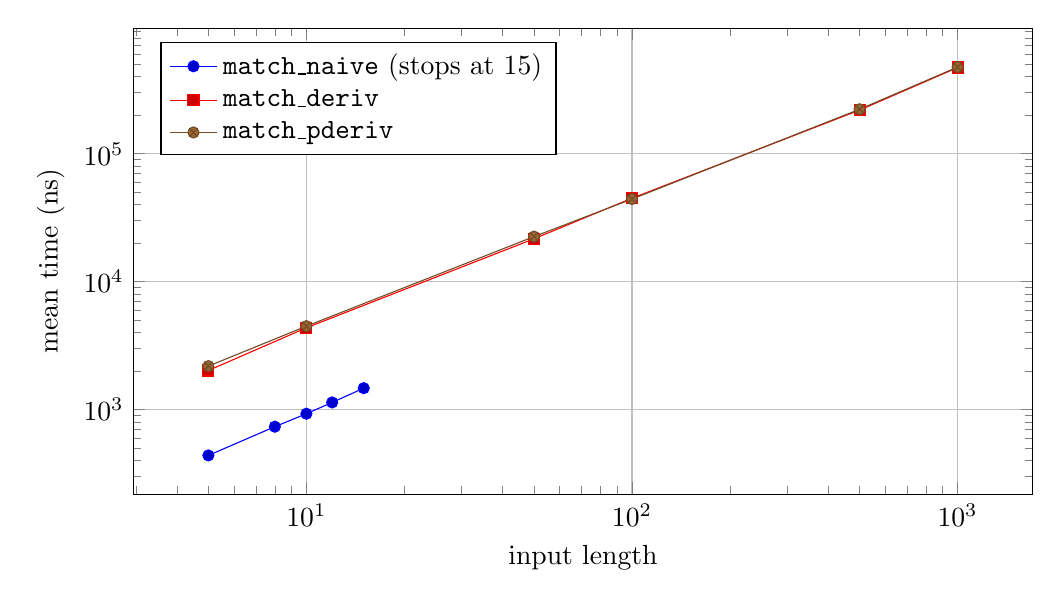
\begin{tikzpicture}
\begin{axis}[
  width=13cm, height=7.5cm,
  xlabel={input length}, ylabel={mean time (ns)},
  xmode=log, ymode=log,
  legend pos=north west, legend cell align=left,
  grid=major,
]
\addplot coordinates {(5,438.9) (8,736.1) (10,929.6) (12,1139) (15,1472)};
\addlegendentry{\texttt{match\_naive} (stops at 15)}
\addplot coordinates {(5,2024) (10,4363) (50,21653) (100,44934) (500,219540) (1000,471765)};
\addlegendentry{\texttt{match\_deriv}}
\addplot coordinates {(5,2189) (10,4495) (50,22518) (100,44276) (500,222756) (1000,476212)};
\addlegendentry{\texttt{match\_pderiv}}
\end{axis}
\end{tikzpicture}
\end{center}

\texttt{match\_naive} is not merely truncated in this plot for space --
it was not benchmarked past length 15 in \texttt{bench\_match.rs} itself,
because its own cost curve on this pattern is already exponential at
that scale; \texttt{match\_deriv}/\texttt{match\_pderiv} are, by
contrast, benchmarked out to length $1000$ in the same group with no
comparable difficulty, tracking each other closely throughout (both
simplify away the same $(a^{*})^{*}$-style redundancy
Section~\ref{sec:simplification-rules-theory} discusses) and growing
roughly linearly rather than exponentially with input length. This is
the central
practical claim Chapter~\ref{sec:motivation} makes for derivative-based
algorithms generally, made directly measurable here rather than left as
an asymptotic argument alone: unlike a backtracking engine
(Section~\ref{sec:motivation}), none of \texttt{match\_naive}'s
better-behaved counterparts -- the two Boolean matchers here, and, on
this specific $(a^{*})^{*}$-shaped input, all four parsers -- exhibit
input-dependent catastrophic blowup. This does \emph{not} generalize to
every pattern: \texttt{docs/DERIV\_BC.md} documents a genuine exception,
found and verified directly rather than assumed absent, where
\texttt{deriv\_bc} specifically -- not the other three parsers -- blows
up on a \emph{different} adversarial pattern, $(a+aa)^{*}$, because that
pattern's ambiguity survives \texttt{simp}'s dedup (which is bit-inclusive,
faithful to Figure 6's own \texttt{nub}, not a shape-only comparison) at
every one of its exponentially many decompositions; the resulting
right-associative \texttt{Alt} chain overflows the stack around $n=20$-$22$.
Antimirov's finiteness bound
(Section~\ref{sec:antimirov-partial-derivatives}) guarantees the
\emph{partial}-derivative parsers stay bounded in exactly this sense --
verified for $(a+aa)^{*}$ specifically in
Section~\ref{sec:ambiguous-star-results} below -- but no equivalent bound
is claimed or proven for \texttt{deriv\_bc}'s bit-annotated simplification
against maximally-ambiguous alternation; the paper itself leaves space
complexity as future work (Section~\ref{sec:bitcoded-optimization-theory}),
and this is exactly the kind of pattern that gap leaves open.

\subsection{Benchmark Results}
\label{sec:benchmark-results}

Three Criterion benchmark suites cover the ground above, plus one more
run against the real-world corpus of Section~\ref{sec:dataset-preparation}
rather than synthetic patterns: \texttt{bench\_match} (the three Boolean
matchers, Section~\ref{sec:pathological-inputs}), \texttt{bench\_posix}
(all five parsing constructions, Section~\ref{sec:deriv-vs-pderiv-performance}),
and \texttt{bench\_dataset}
(\texttt{benches/bench\_dataset.rs}), which runs every parser against a
60-pattern sample of \texttt{data/corpus\_patterns.txt} under several
probe strings, plus a worst-case probe deliberately chosen to contain no
substring any sampled pattern is likely to match early. Real dataset
patterns, run unanchored the way Section~\ref{sec:dataset-preparation}
requires, are measurably bigger and more ambiguous than the hand-built
patterns of \texttt{bench\_posix} alone, which is precisely why this
third suite exists rather than treating the synthetic benchmarks as
sufficient on their own -- \texttt{cargo bench --bench bench\_dataset}
(or, for a fast correctness-only smoke check with no timing collected,
\texttt{-{}- --test}) reproduces its results directly;
\texttt{docs/testing/BENCHMARKS.md} documents invocation and current dataset
provenance in full.

\paragraph{\texttt{ambiguous\_star\_a\_or\_aa}.}
\label{sec:ambiguous-star-results}
$(a+aa)^{*}$ against a run of $n$ \texttt{a}s, referenced above and in
\texttt{docs/DERIV\_BC.md} -- the sizes here (5, 10, 15, 18) are
deliberately small, capped precisely because \texttt{deriv\_bc} is not
safe past roughly $n=20$ on this pattern:

\begin{center}
\begin{tabular}{lrrrr}
\hline
Parser & $n{=}5$ & $n{=}10$ & $n{=}15$ & $n{=}18$ \\
\hline
\texttt{recursive} (\texttt{deriv\_std}) & 8.0\,\textmu s & 110.7\,\textmu s & 1.427\,ms & 6.052\,ms \\
\texttt{bitcoded} (\texttt{deriv\_bc}) & 11.4\,\textmu s & 183.8\,\textmu s & 4.175\,ms & 49.491\,ms \\
\texttt{pderiv\_bc} & 13.4\,\textmu s & 210.6\,\textmu s & 2.207\,ms & 9.236\,ms \\
\texttt{pderiv\_std} & 22.4\,\textmu s & 323.9\,\textmu s & 3.374\,ms & 14.263\,ms \\
\hline
\end{tabular}
\end{center}

\texttt{bitcoded} is the slowest of the four at every size, not merely
at the largest -- and the gap widens with $n$ (roughly $8\times$ slower
than \texttt{recursive} at $n{=}18$, versus roughly $1.4\times$ at
$n{=}5$), consistent with \texttt{docs/DERIV\_BC.md}'s finding that its
simplification pass cannot collapse this pattern's ambiguity, so its
annotated tree grows Fibonacci-large while the other three constructions
stay comparatively controlled over this size range (though, as
Section~\ref{sec:pathological-inputs} already qualifies, "controlled"
here means merely slower-growing, not unaffected -- all four constructions
are measurably costlier here than on the equally-sized but unambiguous
\texttt{scaling\_a\_star}/\texttt{deep\_expression} patterns above).

\paragraph{\texttt{dataset\_corpus\_sample\_sweep}.} All five parsers
against a $60$-pattern sample of the real-world corpus
(Section~\ref{sec:dataset-preparation}), the two short probe strings
Section~\ref{sec:comparison-existing-engines} also uses:

\begin{center}
\begin{tabular}{lr}
\hline
Parser & Mean time / sweep \\
\hline
\texttt{deriv\_std\_rec} & 1.311\,s \\
\texttt{deriv\_std\_loop} & 1.091\,s \\
\texttt{deriv\_bc} & 643.5\,ms \\
\texttt{pderiv\_bc} & 159.2\,ms \\
\texttt{pderiv\_std} & 158.6\,ms \\
\hline
\end{tabular}
\end{center}

The same ranking as \texttt{deep\_expression} above, on real-world rather
than synthetic patterns: the two partial-derivative parsers fastest and
essentially tied, \texttt{deriv\_bc} next at roughly $4\times$ their
cost, and the two unsimplified \texttt{deriv\_std} variants slowest.
Real-world patterns -- padded with the wildcard runs
Section~\ref{sec:dataset-preparation} describes, and considerably larger
than the hand-built patterns above -- do not change which construction
wins, only how far apart the constructions land.

\paragraph{\texttt{dataset\_worst\_case\_probe}.} A single, deliberately
adversarial probe string (chosen to share no early substring with any
sampled pattern, so no parser can reject quickly) against the ten
largest corpus patterns, run only for \texttt{deriv\_std\_rec} and
\texttt{deriv\_bc} -- the un-simplified and bit-coded ends of the
tree-based pair, chosen "for contrast" per that benchmark function's own
comment:

\begin{center}
\begin{tabular}{lr}
\hline
Parser & Mean time \\
\hline
\texttt{deriv\_std\_rec} & 1.000\,s \\
\texttt{deriv\_bc} & 81.1\,ms \\
\hline
\end{tabular}
\end{center}

A roughly $12\times$ gap -- wider than \texttt{dataset\_corpus\_sample\_sweep}'s
$\sim\!2\times$ gap between the same two constructions -- because a
probe engineered to reject as late as possible is exactly the case where
\texttt{deriv\_std\_rec}'s lack of between-step simplification
(Section~\ref{sec:core-algorithm}) costs the most: every step's
expression keeps growing with nothing collapsing it until the whole
probe has been consumed, where \texttt{deriv\_bc}'s \texttt{simp} keeps
the equivalent annotated expression from growing unboundedly for
patterns without $(a+aa)^{*}$-style adversarial ambiguity.



\section{Comparison with Existing Engines}
\label{sec:comparison-existing-engines}

\subsection{Performance}
\label{sec:performance-comparison}

\texttt{benches/bench\_external.rs} (built only under the
\texttt{external-engines} feature, Section~\ref{sec:compared-engines})
runs all five of this thesis's parsers alongside Rust's \texttt{regex}
crate and RE2 -- in both its default leftmost-first mode
(\texttt{re2\_perl}) and its POSIX leftmost-longest mode
(\texttt{re2\_posix}) -- against the identical 60-pattern sample of the
real-world corpus (Section~\ref{sec:dataset-preparation}) and the same
two probe strings \texttt{bench\_dataset.rs} uses, under the same
unanchored-search semantics (\texttt{docs/SUBSTRING\_SEARCH.md}) on both
sides: \texttt{is\_match}/\texttt{PartialMatch} for the external engines,
\texttt{Option::is\_some()} for this thesis's own parsers. One iteration
is one full sweep over the sample. A representative run:

\begin{center}
\begin{tabular}{lrr}
\hline
Engine & Mean time / sweep & vs.\ \texttt{regex} \\
\hline
\texttt{deriv\_std\_rec} (POSIX, recursive) & 1.503\,s & $\times$1{,}415{,}254 \\
\texttt{deriv\_std\_loop} (POSIX, loop) & 1.218\,s & $\times$1{,}146{,}893 \\
\texttt{deriv\_bc} (POSIX, bit-coded) & 690.74\,ms & $\times$650{,}417 \\
\texttt{pderiv\_bc} (Greedy, bit-coded) & 171.85\,ms & $\times$161{,}815 \\
\texttt{pderiv\_std} (Greedy, tree-injection) & 173.28\,ms & $\times$163{,}167 \\
\hline
\texttt{regex} (Rust crate) & 1.06\,\textmu s & $\times$1 \\
\texttt{re2\_perl} (leftmost-first) & 6.61\,\textmu s & $\times$6.2 \\
\texttt{re2\_posix} (leftmost-longest) & 2.75\,\textmu s & $\times$2.6 \\
\hline
\end{tabular}
\end{center}

(RE2's POSIX mode rejects roughly half the corpus sample outright, since
strict POSIX ERE syntax has neither non-capturing groups nor lazy
quantifiers, both idiomatic in this corpus -- \texttt{re2\_posix}'s
figure above is averaged over fewer patterns than the other seven
columns as a result, a known, verified property of the comparison
documented in \texttt{docs/EXTERNAL\_ENGINES.md} rather than a
discrepancy discovered here.)

\paragraph{The gap to \texttt{regex}/RE2 is five to six orders of
magnitude, and this is not a defect to explain away.} Both external
engines compile a pattern once into a table-driven automaton (a Thompson
NFA for \texttt{regex}, a Thompson NFA lazily determinized to a DFA for
RE2 \citep{re2,cox2007}) and then execute a match as a walk over
precomputed transitions, with no allocation per character. Every parser
in this thesis instead re-derives structure on every character of every
match: \texttt{deriv\_std} builds fresh, heap-allocated \texttt{Regex}
nodes each step (Section~\ref{sec:brzozowski-derivatives}),
\texttt{deriv\_bc} threads a growing bit-vector through an annotated
tree (Section~\ref{sec:bitcoded-optimization-theory}), and both
partial-derivative parsers maintain an explicit frontier of
\texttt{(residual, extra)} pairs
(Section~\ref{sec:partial-derivative-parser-theory}) -- none of this is
compiled away or cached between matches. This is a difference in kind,
not a shortfall in the same kind: a from-scratch implementation of an
academic parsing algorithm walking live tree/bit structures cannot be
expected to approach decades-refined, table-driven production automaton
engines, and this thesis treats the measured gap as evidence of exactly
that difference rather than as a result to be minimized.

\paragraph{The ranking among this thesis's own five parsers matches
theory.} The two Greedy, partial-derivative parsers are fastest by a
wide margin (\textasciitilde172\,ms), \texttt{deriv\_bc} is next at
roughly 4.0$\times$ that cost despite being bit-coded rather than
tree-building, and the two unsimplified \texttt{deriv\_std} variants
are slowest. This is consistent with
Section~\ref{sec:deriv-vs-pderiv-performance}'s synthetic-benchmark
finding that the frontier-based partial-derivative construction avoids
costs the full-derivative construction pays, now confirmed on real-world
patterns rather than only the synthetic \texttt{scaling\_a\_star}/
\texttt{deep\_expression} workloads.

\paragraph{The matcher-vs-parser comparison, redone fairly.} Section~\ref{sec:matcher-benchmark-fairness}
(Chapter~\ref{sec:conclusion}) already argued that comparing
\texttt{regex}/RE2's tree-free \texttt{is\_match} against this thesis's
full parsers overstates the gap for membership-only questions, since
none of the three parse-tree/bit-vector-building parsers is what a pure
yes/no question needs. \texttt{external\_matcher\_sample\_sweep}
reruns the same sweep against \texttt{match\_deriv}/\texttt{match\_pderiv}
(Chapter~\ref{sec:derivatives}) instead:

\begin{center}
\begin{tabular}{lrr}
\hline
Engine & Mean time / sweep & vs.\ \texttt{regex} \\
\hline
\texttt{match\_deriv} & 273.07\,ms & $\times$259{,}815 \\
\texttt{match\_pderiv} & 134.95\,ms & $\times$128{,}397 \\
\hline
\texttt{regex} (Rust crate) & 1.05\,\textmu s & $\times$1 \\
\texttt{re2\_perl} (leftmost-first) & 6.63\,\textmu s & $\times$6.3 \\
\texttt{re2\_posix} (leftmost-longest) & 2.72\,\textmu s & $\times$2.6 \\
\hline
\end{tabular}
\end{center}

Both matchers are faster than their full-parser counterparts above
(\texttt{match\_deriv} against \texttt{deriv\_std\_rec}/\texttt{deriv\_bc},
\texttt{match\_pderiv} against \texttt{pderiv\_bc}/\texttt{pderiv\_std}),
as expected -- no parse tree or bit-vector is built -- but the gap to
\texttt{regex}/RE2 barely narrows in relative terms; it is still five
orders of magnitude, not meaningfully closer to four. This is worth
stating plainly rather than treating as a disappointing result: it
confirms Section~\ref{sec:performance-comparison}'s claim that the gap
is architectural (recompute-per-match versus compiled automaton), not an
artifact of this thesis's parsers doing unnecessary tree-building work
on top of an otherwise-comparable matching core -- removing that
tree-building work helps, measurably, but does not touch the actual
source of the gap.

These numbers also reflect a real, verified fix made during this
thesis's development, not the first implementation tried:
\texttt{match\_pderiv} originally rebuilt and deduplicated a
\texttt{HashSet<Regex>} at every \texttt{Alt}/\texttt{Seq}/\texttt{Star}
node during its own recursive derivative computation, in addition to the
one \texttt{HashSet} its top-level per-character loop already needed for
correctness -- the inner deduplication was redundant with, and
subsumed by, the outer one, so it bought no additional soundness while
still paying to hash every intermediate \texttt{Regex} subtree it built.
Two faster alternatives were tried and rejected before landing on the
fix actually shipped, both found unsafe by testing directly against
$(a+aa)^{*}$ rather than assumed adequate: dropping deduplication
entirely reproduces the exact Fibonacci blowup
Section~\ref{sec:ambiguous-star-results} documents for \texttt{deriv\_bc}
(over two million states by 30 characters); deduplicating once per node
locally, mirroring \texttt{pderiv\_bc}'s own \texttt{nub2}
(Section~\ref{sec:partial-derivative-parser-bitcoded-theory}), very
nearly reproduces it too, since local deduplication within one
\texttt{pderiv} call does not bound the union across the many
\emph{different} states the top-level loop tracks simultaneously.
Removing only the demonstrably redundant inner \texttt{HashSet}, leaving
the top-level one untouched, was both safe (verified identical, bounded
behavior on $(a+aa)^{*}$ up to 200 characters) and measurably faster on
this real-corpus sweep.

\paragraph{What would close some of this gap, and what would not.}
Section~\ref{sec:further-performance-optimizations} discusses concrete,
scoped optimizations -- character-class regex nodes in place of the
98-way literal alternation the wildcard padding of
Section~\ref{sec:dataset-preparation} (\texttt{docs/SUBSTRING\_SEARCH.md})
currently builds, structural sharing via \texttt{Rc} in place of
\texttt{Box} to avoid re-cloning untouched subexpressions on every
derivative step, and memoizing \texttt{deriv}/\texttt{nullable} per
\texttt{(Regex, char)} pair -- each plausible, each still operating
within the "recompute per match" model above. Closing the gap fully
would mean caching and reusing the derivative automaton \emph{across}
matches rather than recomputing it on every one -- effectively compiling
a DFA via derivatives, the approach Owens, Reppy, and Turon formalize and
implement \citep{owens2009}. That is a legitimate, well-established
direction, but a different project from the one this thesis undertakes;
Section~\ref{sec:further-performance-optimizations} discusses it as a
direction rather than a plan.

\subsection{Standardized Benchmarking via rebar}
\label{sec:rebar-comparison}

\texttt{rebar} is a benchmarking harness purpose-built for comparing
regular expression engines on equal footing across language and
implementation boundaries, already covering both Rust's \texttt{regex}
crate and RE2 among many others. The bespoke comparison above answers
the immediate question (how do this thesis's parsers compare on this
project's own corpus and probes) but is neither standardized nor
independently maintained; integrating this thesis's parsers as a
\texttt{rebar} target would place them alongside a much wider set of
existing engines and inputs, and against a methodology outside this
project's own control -- named here as the concrete next step toward a
more rigorous version of Section~\ref{sec:performance-comparison}'s
comparison, not yet started.
